% Options for packages loaded elsewhere
\PassOptionsToPackage{unicode}{hyperref}
\PassOptionsToPackage{hyphens}{url}
\documentclass[
]{article}
\usepackage[margin=0.75in]{geometry}
\usepackage{xcolor}
\usepackage{amsmath,amssymb}
\usepackage{graphicx}
\usepackage{placeins}
\usepackage{pgfplots}
\pgfplotsset{compat=1.18}
\usepgfplotslibrary{fillbetween}
\usetikzlibrary{patterns,shapes.geometric,arrows.meta,positioning,calc}
\setcounter{secnumdepth}{-\maxdimen} % remove section numbering
\usepackage{iftex}
\ifPDFTeX
  \usepackage[T1]{fontenc}
  \usepackage[utf8]{inputenc}
  \usepackage{textcomp} % provide euro and other symbols
\else % if luatex or xetex
  \usepackage{unicode-math} % this also loads fontspec
  \defaultfontfeatures{Scale=MatchLowercase}
  \defaultfontfeatures[\rmfamily]{Ligatures=TeX,Scale=1}
\fi
\usepackage{lmodern}
\ifPDFTeX\else
  % xetex/luatex font selection
\fi
% Use upquote if available, for straight quotes in verbatim environments
\IfFileExists{upquote.sty}{\usepackage{upquote}}{}
\IfFileExists{microtype.sty}{% use microtype if available
  \usepackage[]{microtype}
  \UseMicrotypeSet[protrusion]{basicmath} % disable protrusion for tt fonts
}{}
\makeatletter
\@ifundefined{KOMAClassName}{% if non-KOMA class
  \IfFileExists{parskip.sty}{%
    \usepackage{parskip}
  }{% else
    \setlength{\parindent}{0pt}
    \setlength{\parskip}{6pt plus 2pt minus 1pt}}
}{% if KOMA class
  \KOMAoptions{parskip=half}}
\makeatother
\usepackage{longtable,booktabs,array}
\newcounter{none} % for unnumbered tables
\usepackage{calc} % for calculating minipage widths
% Correct order of tables after \paragraph or \subparagraph
\usepackage{etoolbox}
\makeatletter
\patchcmd\longtable{\par}{\if@noskipsec\mbox{}\fi\par}{}{}
\makeatother
% Allow footnotes in longtable head/foot
\IfFileExists{footnotehyper.sty}{\usepackage{footnotehyper}}{\usepackage{footnote}}
\makesavenoteenv{longtable}
\setlength{\emergencystretch}{3em} % prevent overfull lines
\providecommand{\tightlist}{%
  \setlength{\itemsep}{0pt}\setlength{\parskip}{0pt}}
\usepackage[backend=biber,style=authortitle,maxbibnames=99,doi=false,isbn=false,url=true]{biblatex}
\addbibresource{Prohibition_Era_Violence_and_Gangs.bib}
\usepackage{bookmark}
\IfFileExists{xurl.sty}{\usepackage{xurl}}{} % add URL line breaks if available
\urlstyle{same}
\hypersetup{
  hidelinks,
  pdfcreator={LaTeX via pandoc}}

\author{Emmanuel Theodore}
\date{}

\begin{document}

\section{\texorpdfstring{\textbf{The Crucible of Prohibition: Illicit
Markets, Organized Crime, and the Genesis of Federal Gun
Control}}{The Crucible of Prohibition: Illicit Markets, Organized Crime, and the Genesis of Federal Gun Control}}\label{the-crucible-of-prohibition-illicit-markets-organized-crime-and-the-genesis-of-federal-gun-control}

\subsection{\texorpdfstring{\textbf{Introduction: The Architecture of a
Criminogenic
Crisis}}{Introduction: The Architecture of a Criminogenic Crisis}}\label{introduction-the-architecture-of-a-criminogenic-crisis}

The enactment of the Eighteenth Amendment to the United States
Constitution, followed by the enforcement mandates of the National
Prohibition Act (commonly known as the Volstead Act) in 1920, initiated
one of the most profound socio-economic, legal, and criminological
disruptions in modern global history. Driven by the moral and
progressive imperatives of the American Temperance Society, the Women's
Christian Temperance Union, and the Anti-Saloon League, this ``noble
experiment'' sought to eradicate the social and public health ills
associated with alcohol consumption. The theoretical objective was the
purification of American social life, the reduction of domestic
violence, the alleviation of urban poverty, and the promotion of an
efficient, sober industrial workforce. The movement was further
accelerated by the geopolitical environment of World War I, which
fostered a need to conserve grain for troops and catalyzed domestic
hostility toward German-Americans, who were heavily associated with the
domestic brewing industry.\\
However, the practical implementation of Prohibition yielded a
catastrophic policy failure that fundamentally re-engineered the
American criminal landscape. By criminalizing the production,
transportation, and sale of a deeply ingrained cultural commodity for
which there remained a highly inelastic public demand, the state
inadvertently engineered a lucrative, unregulated underground economy of
unprecedented scale. This legislative rupture catalyzed a
multidimensional crisis: it transformed localized, disorganized street
gangs into sophisticated, transnational criminal syndicates; it
generated an unprecedented spike in lethal violence as cartels fought
for market supremacy; and it thoroughly corrupted municipal and federal
law enforcement agencies.\\
Furthermore, the systemic violence generated by this illicit
market---most visibly perpetrated with high-capacity, automatic firearms
such as the Thompson submachine gun---provided the federal government
with the political capital necessary to vastly expand its policing and
regulatory apparatus. Just as the late twentieth-century crack cocaine
epidemic and its corresponding violence were subsequently utilized by
policymakers to justify the mass expansion of the carceral state and the
Violent Crime Control and Law Enforcement Act of 1994, the highly
publicized violence of Alcohol Prohibition was leveraged by the
administration of President Franklin D. Roosevelt to justify the
National Firearms Act of 1934.\\
To research the etiology of Prohibition-era violence and its legislative
aftermath is to recognize a recurring, systemic algorithm in American
public policy: the state enforces a prohibition that inadvertently
births a violent black market, and subsequently weaponizes the violence
generated by that exact market to justify sweeping, permanent expansions
of federal police authority. This report provides an exhaustive,
expert-level diagnostic of this era, analyzing the economic mechanics of
the underground alcohol trade, the professionalization and
multi-generational legacy of criminal cartels, the empirical topography
of the 1920s homicide surge, and the enduring jurisprudential frameworks
of gun control born from the ashes of the Prohibition gang wars.

\subsection{\texorpdfstring{\textbf{The Economics of the Underground:
Bootlegging, Speakeasies, and the Iron Law of
Prohibition}}{The Economics of the Underground: Bootlegging, Speakeasies, and the Iron Law of Prohibition}}\label{the-economics-of-the-underground-bootlegging-speakeasies-and-the-iron-law-of-prohibition}

When the Volstead Act officially took effect on January 17, 1920, it
immediately mandated the closure of thousands of legal saloons,
breweries, and distilleries across the United States. However, the
legislation did not eliminate the public's desire for alcohol; it merely
transferred the entirety of the supply chain from regulated, taxable
businesses to the criminal underworld. Prohibition created a natural
monopoly for organized crime, uniting disparate groups of men who had
previously fought over minor neighborhood territories in a shared effort
to capitalize on a multi-million dollar logistical vacuum.

\subsubsection{\texorpdfstring{\textbf{The Infrastructure of Bootlegging
and ``Rum
Row''}}{The Infrastructure of Bootlegging and ``Rum Row''}}\label{the-infrastructure-of-bootlegging-and-rum-row}

To satisfy the immense national thirst, a complex logistical
infrastructure rapidly developed. Bootlegging operations varied in scale
from small-time urban distillation networks utilizing hidden ``stills''
to massive, international smuggling rings. One of the most prominent
mechanisms for importing high-quality liquor was the establishment of
``Rum Row.'' This phenomenon consisted of a fleet of floating liquor
stores---heavily loaded supply ships carrying whiskey, rum, and
champagne from Great Britain, Canada, and the West Indies---anchored in
international waters just off the Eastern Seaboard.\\
Initially operating three miles off the coast to remain outside U.S.
legal jurisdiction, the heavily patrolled maritime boundary was
eventually extended to twelve miles through subsequent international
treaties. New York's Rum Row, the largest on either coast, was situated
southeast of Nantucket Island and east of Long Island. Smugglers and
local boat operators, known as ``rumrunners,'' utilized highly modified,
high-horsepower speedboats to outrun the underfunded and over-extended
vessels of the U.S. Coast Guard, ferrying illicit cargo from the mother
ships to hidden drop spots along the coastlines of New Jersey, New York,
and Massachusetts.\\
The cat-and-mouse game on the open water was perilous; rumrunners faced
the constant threat of having their vessels seized and being assessed
staggering \$10,000 fines, while the Coast Guard frequently engaged in
live-fire pursuits. In regions like Cape Cod and Martha's Vineyard,
rumrunners utilized the dense fog, intricate coastal inlets, and night
tides to evade detection, unloading cargo into dories and transferring
it to waiting fleets of trucks on the beaches. Figures such as Captain
Bill McCoy gained national fame operating on Rum Row; McCoy refused to
dilute his imported alcohol, giving rise to the cultural idiom ``the
real McCoy'' to denote genuine, unadulterated quality.

\begin{figure}[htbp]
\centering
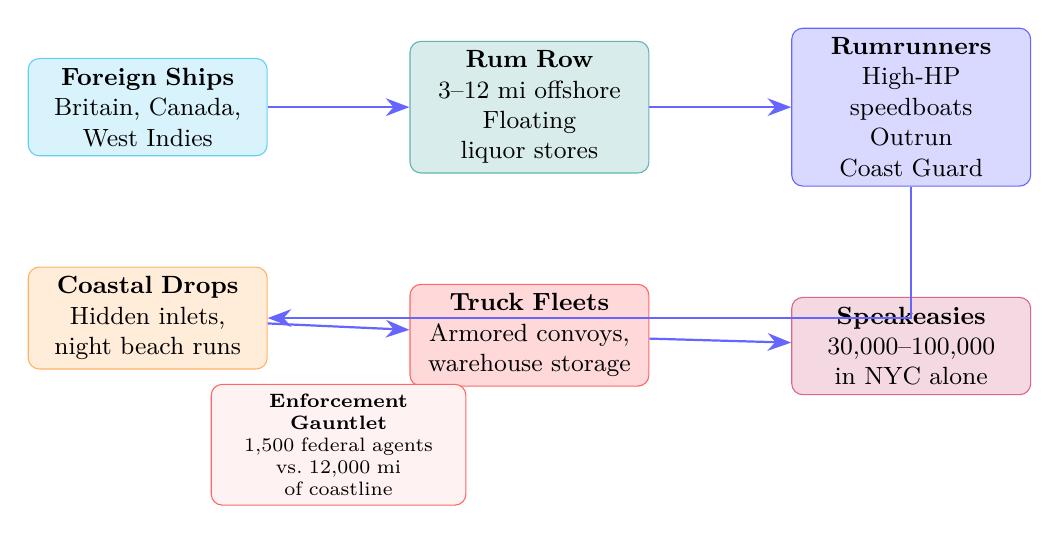
\begin{tikzpicture}[
    node distance=1.4cm and 1.8cm,
    every node/.style={font=\small},
    stage/.style={rectangle, draw=blue!70, fill=blue!10, text width=2.8cm, align=center, rounded corners, minimum height=1.2cm},
    arrow/.style={-{Stealth[length=3mm]}, thick, blue!60},
]
% Nodes
\node[stage, fill=cyan!15, draw=cyan!60] (ships) {\textbf{Foreign Ships}\\Britain, Canada,\\West Indies};
\node[stage, right=of ships, fill=teal!15, draw=teal!60] (rumrow) {\textbf{Rum Row}\\3--12 mi offshore\\Floating liquor stores};
\node[stage, right=of rumrow, fill=blue!15, draw=blue!60] (runners) {\textbf{Rumrunners}\\High-HP speedboats\\Outrun Coast Guard};
\node[stage, below=of ships, fill=orange!15, draw=orange!60] (drops) {\textbf{Coastal Drops}\\Hidden inlets,\\night beach runs};
\node[stage, below=of rumrow, fill=red!15, draw=red!60] (trucks) {\textbf{Truck Fleets}\\Armored convoys,\\warehouse storage};
\node[stage, below=of runners, fill=purple!15, draw=purple!60] (speaks) {\textbf{Speakeasies}\\30,000--100,000\\in NYC alone};

% Arrows
\draw[arrow] (ships) -- (rumrow);
\draw[arrow] (rumrow) -- (runners);
\draw[arrow] (runners) |- (drops);
\draw[arrow] (drops) -- (trucks);
\draw[arrow] (trucks) -- (speaks);

% Threat annotation
\node[rectangle, draw=red!60, fill=red!5, text width=3cm, align=center, font=\scriptsize, rounded corners] at ([yshift=-1.5cm]$(drops)!0.5!(trucks)$) {\textbf{Enforcement Gauntlet}\\1,500 federal agents\\vs.\ 12,000 mi of coastline};
\end{tikzpicture}
\caption{The bootlegging supply chain from international waters to urban speakeasies. The logistical complexity of this pipeline forced criminal gangs to professionalize into corporate-style syndicates. Sources: National Archives; U.S. Coast Guard historical records; The Mob Museum.}
\label{fig:rum-row-supply}
\end{figure}

\subsubsection{\texorpdfstring{\textbf{The Speakeasy and the Subversion
of Cultural
Norms}}{The Speakeasy and the Subversion of Cultural Norms}}\label{the-speakeasy-and-the-subversion-of-cultural-norms}

Once successfully brought onshore, the alcohol was distributed to
private, unlicensed barrooms famously known as ``speakeasies,'' ``blind
pigs,'' or ``gin joints''. The term derived from the necessity for
patrons to speak quietly and provide passwords to gain entry. The scale
of this underground retail network was vast; by 1925, an estimated
30,000 to 100,000 speakeasy clubs were operating in New York City
alone.\\
The speakeasy culture induced a permanent, radical shift in American
social dynamics and gender relations. Prior to Prohibition, drinking in
legal saloons was almost exclusively a male activity, highly segregated
by gender. The illicit, secretive nature of the speakeasy dissolved
these traditional Victorian barriers, creating gender-integrated
environments where men and women drank, socialized, and danced to the
emerging sounds of jazz music. To accommodate female patrons, these
underground restaurants began offering table service and live
entertainment, fueling the cultural explosion of the ``Roaring
Twenties''. The era popularized the modern concept of unsupervised
``dating'' among young adults and empowered the cultural icon of the
``flapper,'' a new generation of women who defied traditional behavioral
constraints.\\
\subsubsection {Toxicity and the ``Iron Law of Prohibition''}
While high-end speakeasies in affluent urban centers served imported, high-quality
liquor from Rum Row, the vast majority of the illicit alcohol consumed
by the working class was domestically produced, often with lethal
consequences. This phenomenon is explained by the ``Iron Law of
Prohibition,'' an economic and pharmacological principle dictating that
as law enforcement pressure against an illicit substance increases, the
potency and toxicity of that substance will inevitably rise.\\
Because bootleggers operated under the constant threat of detection and
seizure, bulky, low-potency beverages like beer and wine became
economically unviable to smuggle, store, or manufacture in massive
quantities. The market organically shifted toward highly concentrated,
easily concealable hard liquors, maximizing the profit-to-volume ratio.
Estimates suggest that the average potency of alcohol products increased
by more than 150 percent during the Prohibition era compared to the
periods immediately preceding and following it.\\
To maximize profit margins, bootleggers frequently adulterated pure
alcohol with water, artificial coloring, and dangerous chemical
additives. The resulting ``rotgut'' or ``bathtub gin'' was often so
foul-tasting that bartenders were forced to invent modern ``cocktails,''
mixing the liquor with ginger ale, sugar, mint, and fruit juices to mask
the flavor. More insidiously, when criminal chemists attempted to
re-distill industrial alcohol---which the federal government had
intentionally poisoned with denaturing additives to prevent human
consumption---the results were catastrophic. Tainted liquors containing
carbolic acid or pure wood alcohol (nicknamed ``Smoke'') caused mass
casualties, killing, blinding, or paralyzing tens of thousands of
Americans during the 1920s. This dynamic perfectly mirrors the
contemporary ``Iron Law'' realities observed in modern drug markets,
where the crackdown on prescription opioids inevitably led to the
dominance of highly potent, highly lethal synthetic fentanyl.

\begin{figure}[htbp]
\centering
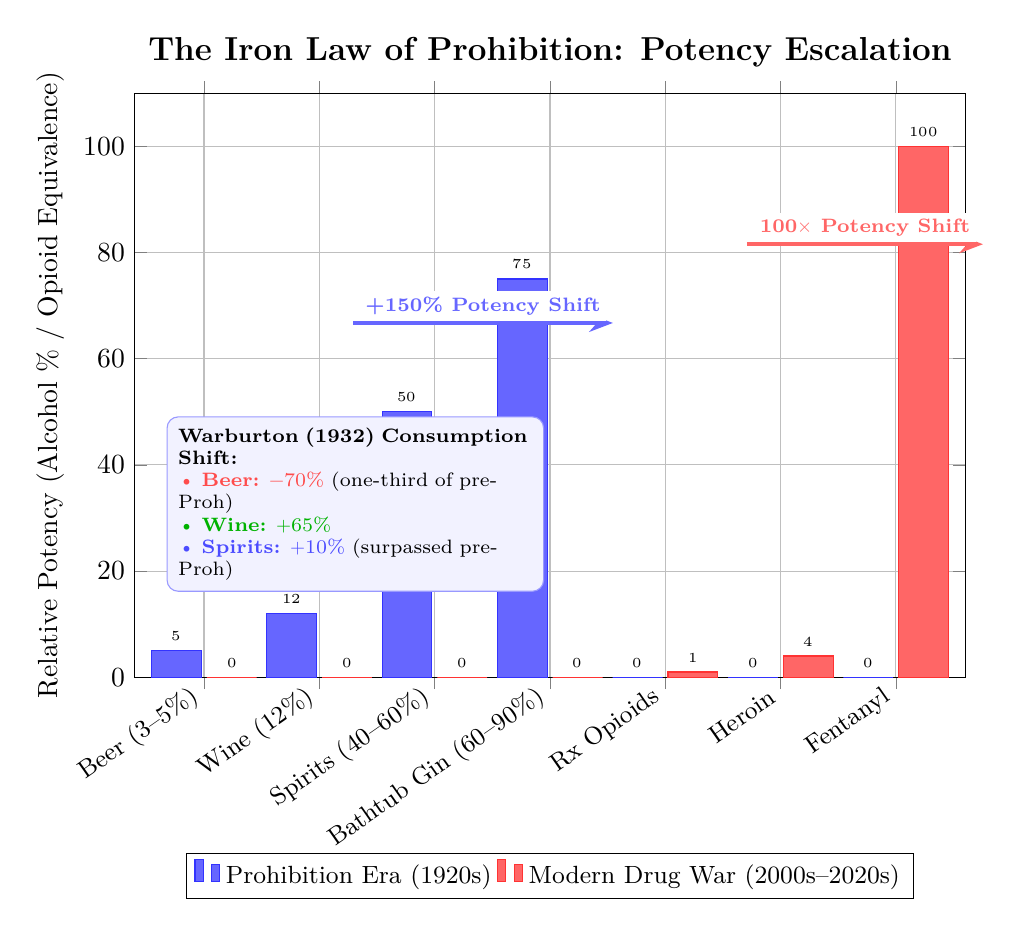
\begin{tikzpicture}
\begin{axis}[
    ybar,
    bar width=18pt,
    width=\textwidth,
    height=9cm,
    ylabel={Relative Potency (Alcohol \% / Opioid Equivalence)},
    symbolic x coords={Beer (3--5\%),Wine (12\%),Spirits (40--60\%),Bathtub Gin (60--90\%),Rx Opioids,Heroin,Fentanyl},
    xtick=data,
    x tick label style={rotate=35, anchor=east, font=\small},
    ymin=0, ymax=110,
    nodes near coords,
    every node near coord/.append style={font=\tiny},
    grid=major,
    title={\textbf{The Iron Law of Prohibition: Potency Escalation}},
    title style={font=\large},
    legend style={at={(0.5,-0.3)}, anchor=north, legend columns=2, font=\small},
]
% Prohibition Era
\addplot[fill=blue!60, draw=blue!80] coordinates {
(Beer (3--5\%),5)
(Wine (12\%),12)
(Spirits (40--60\%),50)
(Bathtub Gin (60--90\%),75)
(Rx Opioids,0)
(Heroin,0)
(Fentanyl,0)
};
% Modern Drug War
\addplot[fill=red!60, draw=red!80] coordinates {
(Beer (3--5\%),0)
(Wine (12\%),0)
(Spirits (40--60\%),0)
(Bathtub Gin (60--90\%),0)
(Rx Opioids,1)
(Heroin,4)
(Fentanyl,100)
};
\legend{Prohibition Era (1920s), Modern Drug War (2000s--2020s)}
\end{axis}

% Annotation arrows
\draw[-{Stealth[length=3mm]}, ultra thick, blue!60] ([xshift=-2.5cm, yshift=4.5cm]current axis.south) -- ([xshift=0.8cm, yshift=4.5cm]current axis.south) node[midway, above, font=\scriptsize\bfseries, fill=white, inner sep=2pt] {+150\% Potency Shift};
\draw[-{Stealth[length=3mm]}, ultra thick, red!60] ([xshift=2.5cm, yshift=5.5cm]current axis.south) -- ([xshift=5.5cm, yshift=5.5cm]current axis.south) node[midway, above, font=\scriptsize\bfseries, fill=white, inner sep=2pt] {100$\times$ Potency Shift};

% Warburton 1932 Consumption Shift Text
\node[text width=4.5cm, align=left, font=\scriptsize, fill=blue!5, draw=blue!40, rounded corners, inner sep=4pt] at ([xshift=2.8cm, yshift=2.2cm]current axis.south west) {
\textbf{Warburton (1932) Consumption Shift:}\\
\textcolor{red!70}{\textbullet\ \textbf{Beer:} $-70\%$} (one-third of pre-Proh)\\
\textcolor{green!70!black}{\textbullet\ \textbf{Wine:} $+65\%$}\\
\textcolor{blue!70}{\textbullet\ \textbf{Spirits:} $+10\%$} (surpassed pre-Proh)
};
\end{tikzpicture}
\caption{The Iron Law of Prohibition dictates that enforcement pressure shifts markets toward maximum potency-per-volume. During Alcohol Prohibition, the market shifted from beer/wine to concentrated spirits and toxic ``bathtub gin'' (150\% average potency increase). The modern War on Drugs replicated this pattern as prescription opioid crackdowns drove the market to heroin and then synthetic fentanyl (50--100$\times$ more potent). Sources: Warburton (1932); Thornton, Cato Institute (1991); DEA National Drug Threat Assessment.}
\label{fig:iron-law}
\end{figure}

\subsection{\texorpdfstring{\textbf{The Metamorphosis of the Syndicate:
From Street Gangs to Organized
Crime}}{The Metamorphosis of the Syndicate: From Street Gangs to Organized Crime}}\label{the-metamorphosis-of-the-syndicate-from-street-gangs-to-organized-crime}

Perhaps the most devastating long-term consequence of the Volstead Act
was its role as a hyper-incubator for modern organized crime. The
architectural evolution of these criminal enterprises fundamentally
altered the American law enforcement landscape for the remainder of the
twentieth century.\\
Prior to 1920, urban criminal gangs existed almost entirely on the
periphery of society. Since the nineteenth century, a social hierarchy
existed wherein big-city ``bosses'' of political machines financed their
control of local wards by accepting payments from criminals running
minor gambling and prostitution rackets, subsequently bribing police to
look the other way. Beneath these political bosses operated fractured,
localized gangs of various ethnic groups---Irish, Italian, Jewish, and
Polish---focused primarily on street-level extortion (such as the
Sicilian ``Black Hand'' rackets), localized loan-sharking, burglary, and
contract violence. These activities were rarely coordinated under a
larger organizational umbrella; indeed, the term ``organized crime'' did
not enter the popular lexicon until the Prohibition era.\\
Prohibition provided these previously fractured groups with an
unprecedented, astronomical economic engine. The logistical demands of
the bootlegging industry---purchasing defunct breweries, acquiring
fleets of armored trucks and speedboats, managing complex international
supply chains, coordinating thousands of speakeasies, and laundering
millions of dollars---required a level of organization that completely
transcended traditional street crime. Criminals were forced to evolve
into corporate executives, employing lawyers, accountants, brewmasters,
and heavily armed enforcers known as ``torpedoes''. The death of a
single leader no longer destroyed the gang; much like a legitimate
corporation, a new executive officer simply stepped into the vacated
position.

\subsubsection{\texorpdfstring{\textbf{The Cartels of Chicago and New
York}}{The Cartels of Chicago and New York}}\label{the-cartels-of-chicago-and-new-york}

In Chicago, the illegal alcohol market was aggressively consolidated by
the Chicago Outfit, a syndicate initially organized by Johnny Torrio and
subsequently inherited by his protégé, Al ``Scarface'' Capone, in 1925
following the violent ``Beer Wars''. Under Capone's ruthless leadership,
the Outfit's operations spanned liquor distribution, speakeasy
ownership, prostitution, and gambling, generating an estimated \$100
million in annual revenue by the late 1920s (equivalent to roughly \$1.4
billion today). Capone secured his empire through staggering systemic
corruption, reportedly distributing \$500,000 monthly to bribe police
officers, judges, and politicians, allowing his organization to operate
with absolute impunity.\\
In New York, a similar professionalization occurred under the guidance
of visionary mobsters like Arnold Rothstein, Meyer Lansky, and Charles
``Lucky'' Luciano. Rothstein, often credited with recognizing the
corporate potential of the underworld, served as a financier and mentor
to younger gangsters, demonstrating how to bridge the gap between street
violence and white-collar commerce. Luciano revolutionized the
structural architecture of the Italian-American Mafia. Recognizing that
continuous, chaotic turf wars disrupted revenue streams, Luciano
orchestrated the assassination of old-guard Sicilian bosses (the
``Mustache Petes'' like Giuseppe Masseria and Salvatore Maranzano). He
reorganized the New York underworld into the ``Five Families'' (Gambino,
Genovese, Lucchese, Bonanno, and Colombo) and established ``The
Commission'' in 1931---a national board of directors composed of crime
family bosses designed to mediate disputes, allocate territories, and
coordinate operations across ethnic lines.

\subsubsection{\texorpdfstring{\textbf{The New England Ecosystem: A
Generational Case
Study}}{The New England Ecosystem: A Generational Case Study}}\label{the-new-england-ecosystem-a-generational-case-study}

The evolution of organized crime was not limited to the primary hubs of
Chicago and New York; it profoundly altered regional ecosystems, as
vividly illustrated by the history of Boston and the broader New England
area. Analyzing the gang structures of Massachusetts provides a perfect
case study of how Prohibition forged criminal empires that dominated the
region for decades.\\
In the early phases of Prohibition, the Boston underworld was dominated
by the Gustin Gang, an Irish-American syndicate led by Frank Wallace and
his brothers Steve and Jim. Originating in the mid-1910s as the
``Tailboard Thieves'' who looted delivery trucks at intersections in
South Boston (``Southie''), the Gustin Gang transitioned aggressively
into the bootlegging trade in the 1920s. Lacking the massive capital,
international connections, and extensive shipping fleets of other
syndicates, the Wallace brothers relied heavily on brute force,
extortion, and ingenuity. They frequently engaged in high-stakes
hijacking, utilizing counterfeit badges resembling those of federal
Prohibition agents to easily confiscate alcohol shipments from rival
bootleggers. They subsequently delivered these stolen shipments to their
own networks, including a speakeasy owned by their older brother Billy
Wallace, known as ``The Sportlight,'' located on Old Colony Avenue.\\
The Gustin Gang operated with a startling degree of legal immunity
throughout the 1920s. Despite being arrested more than 25 times for
offenses ranging from armed robbery to assault and battery, Frank
Wallace rarely served prison time. This immunity was secured through
deep, systemic political corruption; one of the gang's primary attorneys
was John W. McCormack, a powerful state senator who would later become
the Speaker of the United States House of Representatives.\\
However, the localized dominance of the Irish gangs was eventually
eclipsed by the superior organization, ruthlessness, and financial
leverage of Italian-American and Jewish factions. In December 1931, the
reign of the Gustin Gang ended abruptly when Frank Wallace and his
lieutenant Bernard ``Dodo'' Walsh were ambushed and assassinated during
a ``sit-down'' meeting with Italian gangsters, including Joe Lombardo,
at a North End importing company.\\
The power vacuum left by the collapse of the Gustin Gang allowed other
figures to rise, notably the powerful Jewish mob boss Charles ``King''
Solomon, who controlled vast swaths of Boston's bootlegging, narcotics,
and bail bond rackets. However, the drive toward absolute monopolization
was relentless. Solomon was murdered in 1933 at the behest of Filippo
Buccola, an East Boston mobster seeking total consolidation of the
region's rackets. Buccola's successful elimination of rivals allowed him
to formally merge the Boston Mafia with the Providence, Rhode Island
faction (formerly led by Frank Morelli) in 1932, creating a unified,
highly structured New England crime family.\\
In 1954, Buccola retired to Sicily, officially handing control of this
massive, multi-state enterprise to Raymond Patriarca. Patriarca would
rule the New England underworld with an iron fist for the next three
decades from his headquarters in Providence, utilizing the vast wealth
and structural foundations laid during the bloody bootlegging wars of
the 1920s. The legacy of the Prohibition-era Irish gangs also survived;
the remnants of the Gustin Gang's territory eventually gave rise to the
notorious Winter Hill Gang in the 1960s and 1970s, led by figures like
James ``Buddy'' McLean, Howie Winter, and eventually James ``Whitey''
Bulger, who engaged in a multi-decade war with the Patriarca family.
Thus, the territorial lines and gangland rivalries that defined New
England through the end of the 20th century were the direct, downstream
results of the illicit alcohol markets forged in the 1920s.

\subsection{\texorpdfstring{\textbf{The Empirical Topography of
Prohibition-Era
Violence}}{The Empirical Topography of Prohibition-Era Violence}}\label{the-empirical-topography-of-prohibition-era-violence}

Because participants in an illicit black market are fundamentally
excluded from the state's legal mechanisms for dispute resolution---they
cannot sue a supplier for breach of contract, nor call the police if
their inventory is stolen---violence becomes the mandatory, structural
mechanism for enforcing contracts, collecting debts, and protecting
market share. During the Prohibition era, this reliance on ``competitive
violence'' caused a staggering surge in the national homicide rate,
mirroring the later spikes seen during the 1980s crack cocaine epidemic.

\subsubsection{\texorpdfstring{\textbf{Statistical Trajectories of
Lethal
Violence}}{Statistical Trajectories of Lethal Violence}}\label{statistical-trajectories-of-lethal-violence}

Analyzing crime data from the early twentieth century presents distinct
methodological challenges, as the FBI's Uniform Crime Reporting (UCR)
program was not standardized until 1930, and early state-level reporting
was highly fragmented. However, utilizing reconstructed historical
census data, vital health statistics, and localized datasets,
criminologists and historians have mapped a clear, undeniable trajectory
of violence directly corresponding to the enactment and subsequent
repeal of the 18th Amendment.\\
Prior to the onset of Prohibition, the national homicide rate hovered
consistently between 4.5 and 6 deaths per 100,000 population. Following
the passage of the Volstead Act, this rate began a sustained,
precipitous climb, peaking at an estimated 9.8 to 10 homicides per
100,000 residents in 1933. This represented a massive increase of
roughly 78 percent over the pre-Prohibition baseline.\\
\textbf{Table 1: Estimated U.S. Homicide Trajectory (per 100,000
population), 1910 - 1940}

{\def\LTcaptype{none} % do not increment counter
\begin{longtable}[]{@{}lll@{}}
\toprule\noalign{}
Year / Era & Homicide Rate (per 100,000) & Contextual Notes \\
\midrule\noalign{}
\endhead
\bottomrule\noalign{}
\endlastfoot
1910 & \textasciitilde{} 4.6 & Pre-Prohibition baseline \\
1915 & \textasciitilde{} 5.9 & Pre-Prohibition baseline \\
1920 & \textasciitilde{} 6.8 & First year of National Prohibition \\
1925 & \textasciitilde{} 8.6 & Escalation of gang territorial wars \\
1929 & \textasciitilde{} 8.8 & Year of the St.~Valentine's Day
Massacre \\
1933 & \textasciitilde{} 9.8 & Peak violence; 21st Amendment ratified
(Repeal) \\
1936 & \textasciitilde{} 8.0 & Post-Repeal decline accelerates \\
1940 & \textasciitilde{} 6.2 & Return to near pre-Prohibition levels \\
\end{longtable}
}

\emph{Data synthesized from historical U.S. Vital Statistics, Bureau of
the Census reconstructions, and BJS Homicide Trends.}

\begin{figure}[htbp]
\centering
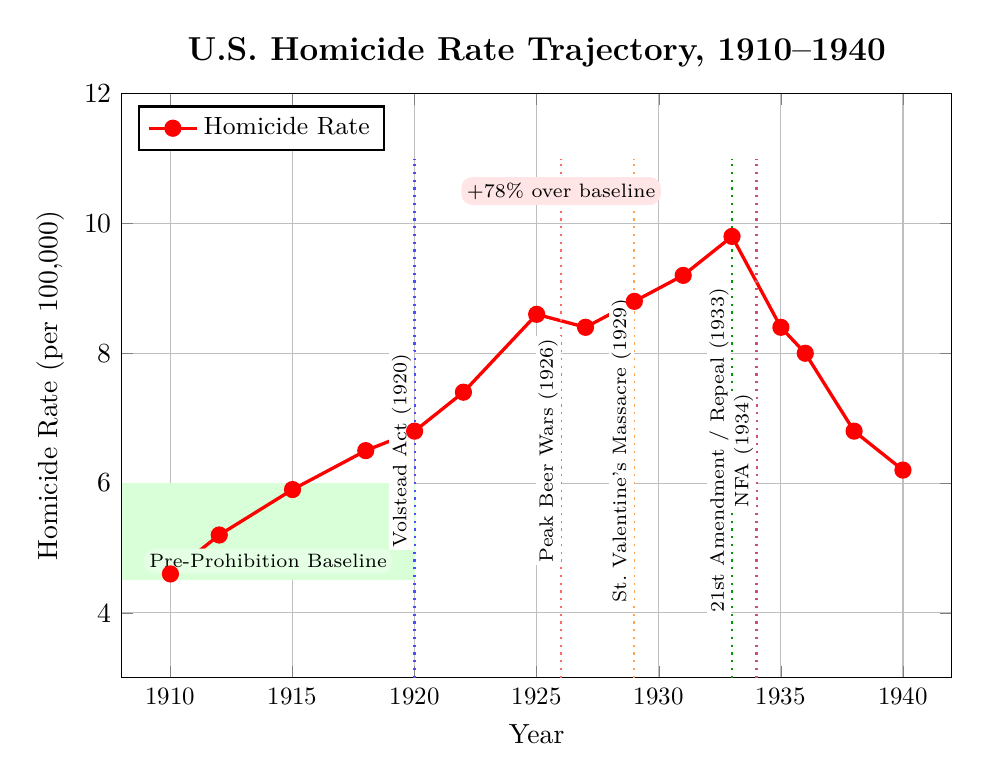
\begin{tikzpicture}
\begin{axis}[
    width=\textwidth,
    height=9cm,
    xlabel={Year},
    ylabel={Homicide Rate (per 100,000)},
    xmin=1908, xmax=1942,
    ymin=3, ymax=12,
    grid=major,
    title={\textbf{U.S. Homicide Rate Trajectory, 1910--1940}},
    title style={font=\large},
    legend style={at={(0.02,0.98)}, anchor=north west, font=\small},
    thick,
    scaled x ticks=false,
    xticklabel style={
      font=\small,
      /pgf/number format/.cd,
      fixed,
      precision=0,
      set thousands separator={},
    },
]
% Homicide rate line
\addplot[color=red, mark=*, mark size=2.5, very thick] coordinates {
(1910,4.6)
(1912,5.2)
(1915,5.9)
(1918,6.5)
(1920,6.8)
(1922,7.4)
(1925,8.6)
(1927,8.4)
(1929,8.8)
(1931,9.2)
(1933,9.8)
(1935,8.4)
(1936,8.0)
(1938,6.8)
(1940,6.2)
};
\addlegendentry{Homicide Rate}

% Pre-Prohibition baseline band
\addplot[name path=baseline_top, draw=none] coordinates {(1908,6)(1920,6)};
\addplot[name path=baseline_bot, draw=none] coordinates {(1908,4.5)(1920,4.5)};
\addplot[fill=green!15] fill between[of=baseline_top and baseline_bot];

% Policy annotations
\draw[dotted, thick, blue!70] (axis cs:1920,3) -- (axis cs:1920,11);
\node[rotate=90, anchor=south, font=\scriptsize, fill=white, inner sep=1pt] at (axis cs:1920,6.5) {Volstead Act (1920)};

\draw[dotted, thick, red!60] (axis cs:1926,3) -- (axis cs:1926,11);
\node[rotate=90, anchor=south, font=\scriptsize, fill=white, inner sep=1pt] at (axis cs:1926,6.5) {Peak Beer Wars (1926)};

\draw[dotted, thick, orange!70] (axis cs:1929,3) -- (axis cs:1929,11);
\node[rotate=90, anchor=south, font=\scriptsize, fill=white, inner sep=1pt] at (axis cs:1929,6.5) {St.\ Valentine's Massacre (1929)};

\draw[dotted, thick, green!60!black] (axis cs:1933,3) -- (axis cs:1933,11);
\node[rotate=90, anchor=south, font=\scriptsize, fill=white, inner sep=1pt] at (axis cs:1933,6.5) {21st Amendment / Repeal (1933)};

\draw[dotted, thick, purple!70] (axis cs:1934,3) -- (axis cs:1934,11);
\node[rotate=90, anchor=south, font=\scriptsize, fill=white, inner sep=1pt] at (axis cs:1934,6.5) {NFA (1934)};

% Annotations
\node[font=\scriptsize, fill=green!10, rounded corners, inner sep=2pt] at (axis cs:1914,4.8) {Pre-Prohibition Baseline};
\node[font=\scriptsize, fill=red!10, rounded corners, inner sep=2pt] at (axis cs:1926,10.5) {+78\% over baseline};
\end{axis}
\end{tikzpicture}
\caption{U.S. homicide rate trajectory showing the direct correspondence between Prohibition (1920--1933) and the surge in lethal violence. The rate climbed 78\% above pre-Prohibition baselines, peaking in 1933, then fell sharply following Repeal. The green band indicates the pre-Prohibition baseline range (4.5--6.0 per 100,000). Sources: BJS Homicide Trends; CDC Vital Statistics; Bureau of the Census reconstructions.}
\label{fig:homicide-rate}
\end{figure}

The sheer volume of urban violence was staggering. In 1926 alone, more
than 12,000 murders were recorded across the United States. While some
contemporaries argued that the perceived ``crime wave'' was merely media
sensationalism, detailed analyses prove that while minor public order
offenses (such as vagrancy or public swearing) decreased, severe violent
crimes skyrocketed. Between 1910 and 1923, national robbery rates surged
by 83.3 percent, and homicides increased by 16.1 percent, directly
correlating with the rise of the illegal traffic.

\subsubsection{\texorpdfstring{\textbf{Systemic
vs.~Psychopharmacological
Violence}}{Systemic vs.~Psychopharmacological Violence}}\label{systemic-vs.-psychopharmacological-violence}

A rigorous epidemiological analysis of the Chicago Historical Homicide
Project---a dataset chronicling 11,018 homicides between 1870 and
1930---reveals the precise nature of this violence. Using interrupted
time-series and ARIMA models, researchers demonstrated that during
Prohibition, total homicides in Chicago increased by 21 percent, and
non-alcohol-related homicides increased by 11 percent. Crucially, the
rate of homicides committed by individuals under the direct influence of
alcohol remained statistically unchanged throughout the era.\\
This divergence is analytically profound. It proves that the surge in
murders was not the ``psychopharmacological'' result of citizens
becoming intoxicated and violent, but rather the structural byproduct of
intense, competitive market violence between rival bootlegging factions
fighting for control of distribution networks.\\
Public health scholarship further corroborates the continued consumption
of alcohol despite the ban. In New Orleans, despite Prohibition
enforcement, the death rate from liver cirrhosis rose by 25.1 percent
between 1920 and 1929, indicating that massive quantities of toxic
illicit alcohol were still being consumed. Yet, when Prohibition ended
in 1933, the cirrhosis death rate plummeted by 34.7 percent over the
next decade as the market re-regulated, mirroring the simultaneous,
steep collapse in the national homicide rate.

\begin{figure}[htbp]
\centering
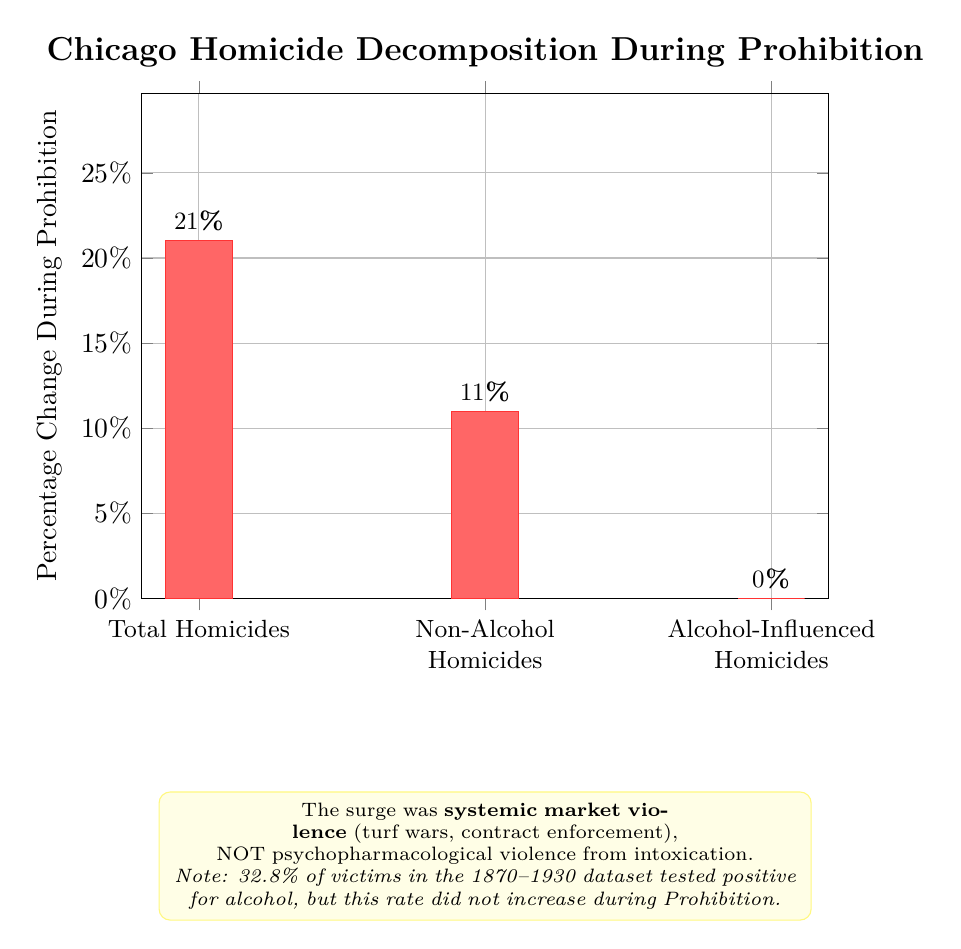
\begin{tikzpicture}
\begin{axis}[
    ybar,
    bar width=24pt,
    width=0.85\textwidth,
    height=8cm,
    ylabel={Percentage Change During Prohibition},
    symbolic x coords={Total Homicides,Non-Alcohol Homicides,Alcohol-Influenced Homicides},
    xtick=data,
    x tick label style={text width=3cm, align=center, font=\small},
    ymin=0, ymax=28,
    enlarge y limits={value=0.06, upper},
    nodes near coords={\pgfmathprintnumber\pgfplotspointmeta\%},
    every node near coord/.append style={font=\small\bfseries},
    grid=major,
    title={\textbf{Chicago Homicide Decomposition During Prohibition}},
    title style={font=\large},
    ytick={0,5,10,15,20,25},
    yticklabel={\pgfmathprintnumber\tick\%},
]
\addplot[fill=red!60, draw=red!80] coordinates {
(Total Homicides,21)
(Non-Alcohol Homicides,11)
(Alcohol-Influenced Homicides,0)
};
\end{axis}
\node[anchor=north, text width=8cm, align=center, font=\scriptsize, fill=yellow!10, draw=yellow!50, rounded corners, inner sep=4pt] at ([yshift=-2.45cm]current axis.south) {The surge was \textbf{systemic market violence} (turf wars, contract enforcement),\\NOT psychopharmacological violence from intoxication.\\\textit{Note: 32.8\% of victims in the 1870--1930 dataset tested positive for alcohol, but this rate did not increase during Prohibition.}};
\end{tikzpicture}
\caption{Decomposition of the Prohibition-era homicide increase in Chicago (1870--1930 dataset, 11,018 cases). The 21\% total increase was driven entirely by non-alcohol-related systemic violence between rival bootlegging factions, while homicides committed under the influence of alcohol remained statistically unchanged --- proving the violence was a structural market output, not a behavioral consequence of intoxication. Source: Asbridge \& Weerasinghe (2009), Chicago Historical Homicide Project; ARIMA time-series analysis.}
\label{fig:chicago-decomposition}
\end{figure}

\subsection{\texorpdfstring{\textbf{Enforcement Asymmetries and the
Failure of the
State}}{Enforcement Asymmetries and the Failure of the State}}\label{enforcement-asymmetries-and-the-failure-of-the-state}

The inability of the state to curb the rising tide of violence was
rooted in a profound asymmetry of resources, training, and systemic
integrity. The National Prohibition Act tasked the commissioner of the
Internal Revenue Service (IRS) within the Treasury Department with
overseeing enforcement. The IRS established the Prohibition Unit,
initially deploying a meager force of only 1,500 agents to police the
entire geography of the United States---encompassing 12,000 miles of
shoreline, 3,900 miles of international borders, and a population eager
to consume alcohol.\\
The enforcement apparatus was chronically underfunded; in 1923, the
federal government and states combined spent less than \$500,000 on
enforcement efforts. Furthermore, Prohibition agents (nicknamed
``Prohis'') were initially exempt from Civil Service exam requirements,
leading to rampant political cronyism and the hiring of agents with
highly questionable backgrounds. Issued firearms but lacking formal
training, these agents were highly susceptible to corruption. Given that
an agent's salary ranged from a paltry \$1,200 to \$3,000 annually, the
temptation to accept bribes from bootleggers generating millions was
irresistible. By 1930, 1,587 federal Prohibition employees had been
officially terminated for offenses including perjury, robbery, bribery,
and embezzlement.\\
Despite the systemic rot, certain federal actors achieved legendary
status through innovative, albeit insufficient, enforcement tactics.
Agents Izzy Einstein and Moe Smith became national sensations by
utilizing elaborate theatrical disguises---posing as firemen,
gravediggers, and football players---to infiltrate and raid thousands of
speakeasies in New York. In Chicago, Special Agent Eliot Ness famously
assembled a handpicked detail of incorruptible agents, dubbed the
``Untouchables,'' to physically dismantle Al Capone's illicit breweries
and distribution networks.\\
Ultimately, traditional law enforcement tactics proved inadequate
against deeply entrenched syndicates. The federal government was forced
to pivot its legal strategy. Led by Elmer Irey of the Special
Intelligence Unit, the Treasury Department utilized a 1927 Supreme Court
ruling (the Manly Sullivan case), which determined that illegal income
was subject to federal income tax. By deploying forensic accountants to
track money laundering, the federal government successfully prosecuted
Al Capone not for bootlegging or murder, but for felony tax evasion,
sentencing him to 11 years in federal prison in 1931.

\begin{figure}[htbp]
\centering
\hspace*{-0.04\textwidth}%
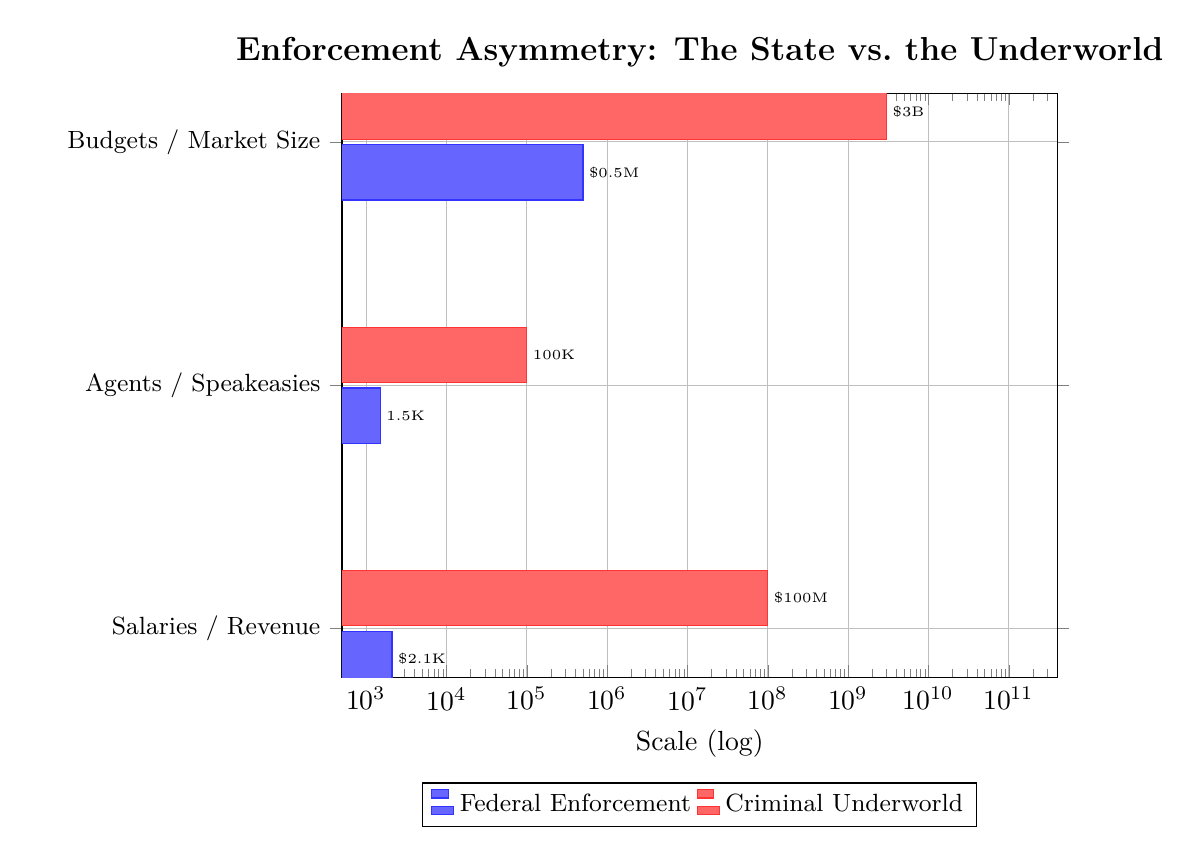
\begin{tikzpicture}
\begin{axis}[
    xbar,
    bar width=20pt,
    width=0.88\textwidth,
    height=9cm,
    xlabel={Scale (log)},
    xmode=log,
    xmin=500, xmax=10000000000,
    enlarge x limits={0.22, upper},
    symbolic y coords={Salaries / Revenue,Agents / Speakeasies,Budgets / Market Size},
    ytick=data,
    y tick label style={font=\small, text width=3.6cm, align=right},
    nodes near coords,
    every node near coord/.append style={font=\tiny, anchor=west, inner xsep=2pt},
    point meta=explicit symbolic,
    grid=major,
    title={\textbf{Enforcement Asymmetry: The State vs.\ the Underworld}},
    title style={font=\large},
    legend style={at={(0.5,-0.18)}, anchor=north, legend columns=2, font=\small},
]
% Federal Enforcement
\addplot[fill=blue!60, draw=blue!80] coordinates {
(2100,Salaries / Revenue) [\$2.1K]
(1500,Agents / Speakeasies) [1.5K]
(500000,Budgets / Market Size) [\$0.5M]
};

% Criminal Underworld
\addplot[fill=red!60, draw=red!80] coordinates {
(100000000,Salaries / Revenue) [\$100M]
(100000,Agents / Speakeasies) [100K]
(3000000000,Budgets / Market Size) [\$3B]
};
\legend{Federal Enforcement, Criminal Underworld}
\end{axis}
\end{tikzpicture}
\caption{The structural asymmetry between federal enforcement resources and the scale of the illicit alcohol economy. With only 1,500 agents earning \$1,200--\$3,000 annually and a combined enforcement budget under \$500,000, the state was outmatched by an underground economy generating over \$100 million annually for a single syndicate. By 1930, 1,587 agents had been terminated for corruption. Sources: Prohibition Bureau records; Cato Institute (1991); DOJ historical reports.}
\label{fig:enforcement-asymmetry}
\end{figure}

\subsection{\texorpdfstring{\textbf{The Catalyst of Atrocity: The
St.~Valentine's Day
Massacre}}{The Catalyst of Atrocity: The St.~Valentine's Day Massacre}}\label{the-catalyst-of-atrocity-the-st.-valentines-day-massacre}

While statistical data outlines the macro-level tragedy of the era, the
political and cultural shift regarding Prohibition was driven by highly
visible, spectacular acts of public violence. The apex of this
brutality---and the catalyst for sweeping federal legislative
reform---occurred on the morning of February 14, 1929, in an event
universally known as the St.~Valentine's Day Massacre.\\
In Chicago, the vicious territorial rivalry between Al Capone's Italian
South Side Outfit and George ``Bugs'' Moran's predominantly Irish North
Side Gang had raged for years, resulting in hundreds of mobster and
police casualties. Seeking to permanently eradicate Moran's operation,
Capone's associates orchestrated a meticulously planned ambush.\\
Seven members and associates of the North Side Gang were lured to a
garage at 2122 N. Clark Street under the pretense of receiving a
hijacked, discounted shipment of imported whiskey. Four men---two of
whom were dressed in stolen Chicago Police Department uniforms---entered
the garage, ordered the men to line up facing the rear brick wall, and
executed them. The executioners utilized two Thompson submachine guns
and two shotguns, unleashing a devastating barrage of 70 rounds into the
victims' backs and heads.\\
Although Moran himself narrowly escaped (having arrived late and spotted
the ``police'' entering), his criminal empire was effectively crippled.
Capone, who conveniently established a highly public alibi by
vacationing in Florida, was universally recognized as the architect of
the slaughter, though neither he nor his suspected hitmen (such as Fred
Burke) were ever successfully prosecuted for the massacre.\\
The St.~Valentine's Day Massacre acted as a profound psychological
interface shift for the American electorate. Prior to 1929, many
citizens viewed bootleggers as romanticized, anti-establishment figures
providing a desired service in defiance of an unpopular law. The sheer
barbarity of the garage executions, captured in gruesome press
photographs and disseminated nationally, evaporated this public
sympathy. The massacre forced the federal government to acknowledge that
municipal police forces were entirely outgunned and hopelessly
corrupted, necessitating a highly aggressive, federalized response to
combat organized crime.

\subsection{\texorpdfstring{\textbf{The Legislative Architecture: The
National Firearms Act of
1934}}{The Legislative Architecture: The National Firearms Act of 1934}}\label{the-legislative-architecture-the-national-firearms-act-of-1934}

The extreme violence of the Prohibition era provided the federal state
with the essential political leverage to construct the foundational
architecture of modern American gun control.\\
The signature weapon of the era's gangland warfare was the Thompson
submachine gun. Invented by John T. Thompson in 1918 and originally
intended for trench warfare, the ``Tommy Gun'' fired heavy.45 ACP
ammunition at a cyclic rate of 600 to 900 rounds per minute. Equipped
with 50- or 100-round drum magazines and easily concealable beneath a
top coat, the weapon provided unprecedented, squad-level automatic
firepower to single individuals. Because the weapon was legally
available for commercial purchase by the general public, it was rapidly
adopted by syndicates and bank robbers, earning the grim moniker the
``Chicago Typewriter''.\\
As the national homicide rate climbed to its 1933 peak, and following a
highly publicized assassination attempt on President-elect Franklin D.
Roosevelt in 1933, the newly formed administration declared a national
``War on Crime''. Tasked with dismantling the syndicates, Attorney
General Homer S. Cummings recognized that a patchwork of local
ordinances was entirely insufficient to combat heavily armed, interstate
cartels. Cummings drafted what would become the National Firearms Act
(NFA) of 1934, the first comprehensive federal firearm legislation in
U.S. history.

\subsubsection{\texorpdfstring{\textbf{The Mechanics of the NFA:
Taxation as
Regulation}}{The Mechanics of the NFA: Taxation as Regulation}}\label{the-mechanics-of-the-nfa-taxation-as-regulation}

The legislative strategy behind the NFA was profoundly shaped by the
constitutional constraints of the era. In the 1930s, the prevailing
interpretation of the Second Amendment, combined with strict limits on
the Interstate Commerce Clause, posed significant barriers to an
outright federal ban on firearms. To circumvent this, Cummings and the
Department of Justice ingeniously utilized Congress's enumerated Article
I power to levy taxes.\\
During his testimony before the House Committee on Ways and Means,
Cummings employed highly inflammatory rhetoric to mobilize legislative
action, declaring that the ``armed underworld'' rivaled the size of the
U.S. Army and referring to gangsters as ``predatory criminals'' posing a
``serious national emergency''. When questioned regarding the
constitutionality of the bill by Congressman Hatton Sumners, Cummings
explicitly admitted the legislative sleight-of-hand: ``If we had a
statute absolutely forbidding any human being to have a machine gun, you
might say there is some constitutional question involved. But when you
say, `we will tax the machine gun,' \ldots{} you are easily within the
law''.\\
The original draft of the NFA (H.R. 9066) sought to require registration
and heavy taxation on all concealable firearms, including standard
pistols and revolvers, as well as machine guns. However, intense
lobbying by the National Rifle Association (NRA) forced a critical
compromise; handguns were stripped from the final legislation.\\
The finalized National Firearms Act of 1934 mandated the registration of
specific ``gangster weapons''---defined as machine guns, short-barreled
(sawed-off) rifles and shotguns, and firearm silencers/mufflers---with
the Secretary of the Treasury. The Act imposed a staggering \$200
transfer and making tax on these items. In 1934, when a brand new
Thompson submachine gun cost approximately \$175, the \$200 tax
(equivalent to roughly \$3,600 in modern inflation-adjusted currency)
effectively doubled or tripling the cost of the weapon.\\
\textbf{Table 2: Original NFA Weapon Categorizations and Tax Structures
(1934)}

{\def\LTcaptype{none} % do not increment counter
\begin{longtable}[]{@{}
  >{\raggedright\arraybackslash}p{(\linewidth - 6\tabcolsep) * \real{0.2500}}
  >{\raggedright\arraybackslash}p{(\linewidth - 6\tabcolsep) * \real{0.2500}}
  >{\raggedright\arraybackslash}p{(\linewidth - 6\tabcolsep) * \real{0.2500}}
  >{\raggedright\arraybackslash}p{(\linewidth - 6\tabcolsep) * \real{0.2500}}@{}}
\toprule\noalign{}
\begin{minipage}[b]{\linewidth}\raggedright
Firearm Category
\end{minipage} & \begin{minipage}[b]{\linewidth}\raggedright
Definition Parameters
\end{minipage} & \begin{minipage}[b]{\linewidth}\raggedright
Regulatory Action
\end{minipage} & \begin{minipage}[b]{\linewidth}\raggedright
Purpose / Target Demographic
\end{minipage} \\
\midrule\noalign{}
\endhead
\bottomrule\noalign{}
\endlastfoot
\textbf{Machine Guns} & Any weapon shooting automatically more than one
shot without manual reloading. & \$200 Tax + Registration & Target
cartel enforcers (Thompson SMG). \\
\textbf{Short-Barreled Shotguns} & Shotgun having a barrel less than 18
inches in length. & \$200 Tax + Registration & Target easily concealable
bank robbery tools. \\
\textbf{Short-Barreled Rifles} & Rifle having a barrel less than 16
inches in length. & \$200 Tax + Registration & Target easily concealable
long guns. \\
\textbf{Silencers/Mufflers} & Device for silencing, muffling, or
diminishing the report of a portable firearm. & \$200 Tax + Registration
& Target assassination tools used by hitmen. \\
\textbf{Pistols/Revolvers} & Standard handguns. & \emph{Removed from
Bill} & Originally targeted, removed via NRA lobbying. \\
\end{longtable}
}

\begin{figure}[htbp]
\centering
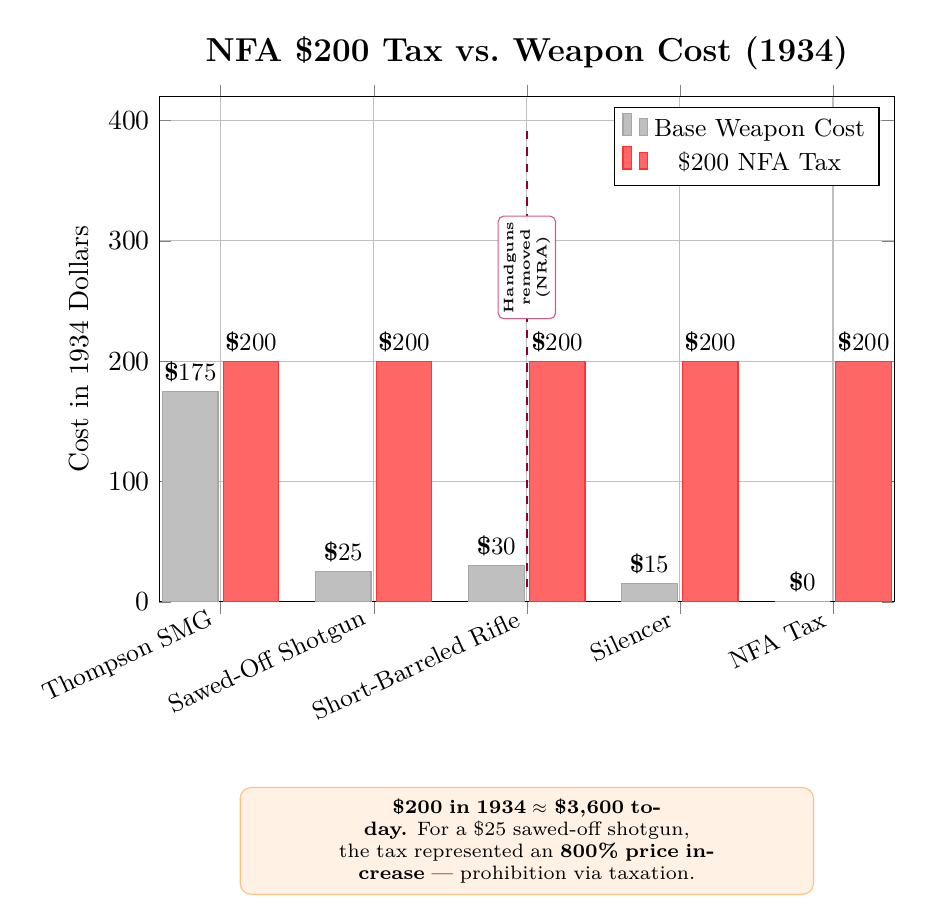
\begin{tikzpicture}
\begin{axis}[
    ybar,
    bar width=20pt,
    width=0.9\textwidth,
    height=8cm,
    ylabel={Cost in 1934 Dollars},
    symbolic x coords={Thompson SMG,Sawed-Off Shotgun,Short-Barreled Rifle,Silencer,NFA Tax},
    xtick=data,
    x tick label style={rotate=25, anchor=east, font=\small},
    ymin=0, ymax=420,
    nodes near coords={\$\pgfmathprintnumber\pgfplotspointmeta},
    every node near coord/.append style={font=\small\bfseries},
    grid=major,
    title={\textbf{NFA \$200 Tax vs.\ Weapon Cost (1934)}},
    title style={font=\large},
    legend style={at={(0.98,0.98)}, anchor=north east, font=\small},
]
% Weapon base cost
\addplot[fill=gray!50, draw=gray!70] coordinates {
(Thompson SMG,175)
(Sawed-Off Shotgun,25)
(Short-Barreled Rifle,30)
(Silencer,15)
(NFA Tax,0)
};
% NFA Tax overlay
\addplot[fill=red!60, draw=red!80] coordinates {
(Thompson SMG,200)
(Sawed-Off Shotgun,200)
(Short-Barreled Rifle,200)
(Silencer,200)
(NFA Tax,200)
};
\legend{Base Weapon Cost, \$200 NFA Tax}
\pgfplotsextra{%
  \draw[dashed, purple!75!black, line width=0.9pt] (axis cs:{Short-Barreled Rifle},12) -- (axis cs:{Short-Barreled Rifle},398);
  \node[rotate=90, anchor=center, font=\tiny\bfseries, text=black, fill=white, fill opacity=0.94, draw=purple!65, rounded corners=2pt, inner sep=2pt, align=center] at (axis cs:{Short-Barreled Rifle},278) {Handguns\\removed\\(NRA)};
}
\end{axis}
\node[anchor=north, text width=7cm, align=center, font=\scriptsize, fill=orange!10, draw=orange!50, rounded corners, inner sep=4pt] at ([yshift=-2.35cm]current axis.south) {\textbf{\$200 in 1934 $\approx$ \$3,600 today.} For a \$25 sawed-off shotgun,\\the tax represented an \textbf{800\% price increase} --- prohibition via taxation.};
\end{tikzpicture}
\caption{The NFA's \$200 transfer tax shown against the base cost of each regulated weapon category. The tax effectively doubled the cost of a Thompson submachine gun and increased the cost of cheaper weapons by 670--1,300\%, achieving \emph{de facto} prohibition through prohibitive pricing. Handguns were originally included but removed via NRA lobbying. Sources: ATF NFA historical records; House Ways and Means Committee hearings (1934).}
\label{fig:nfa-tax}
\end{figure}

The underlying purpose of the NFA was explicitly not revenue collection,
but absolute prohibition via prohibitive pricing and strict registration
requirements (which included fingerprinting and photographing
applicants). As Cummings intended, while wealthy cartel bosses like
Capone could easily afford the \$200 tax, they actively avoided
registration to prevent providing federal agents with documented proof
of their identities, locations, and arsenals. Consequently, the mere
possession of an unregistered NFA weapon became a federal felony,
providing the fledgling FBI and Treasury agents with a powerful legal
mechanism to arrest and imprison mobsters when underlying charges of
murder or extortion could not be proven in local courts.\\
The NFA faced subsequent legal challenges, but its framework was upheld
by the Supreme Court in cases such as \emph{Sonzinsky v. United States}
(1937), which validated the taxing mechanism, and \emph{United States v.
Miller} (1939), which ruled that the Second Amendment did not protect
weapons (like sawed-off shotguns) that lacked a reasonable relationship
to the preservation of a well-regulated militia. The success of the NFA
in practically eliminating the legal commercial market for fully
automatic weapons established a durable jurisprudential architecture. By
successfully utilizing the tax code to enact sweeping social control,
the Roosevelt administration set a profound legal precedent that would
shortly be used to draft the Marihuana Tax Act of 1937, officially
launching the federal war on drugs using the exact same constitutional
mechanism.

\subsection{\texorpdfstring{\textbf{Retrospective Diagnostics: Repeal
and the Post-Prohibition
Landscape}}{Retrospective Diagnostics: Repeal and the Post-Prohibition Landscape}}\label{retrospective-diagnostics-repeal-and-the-post-prohibition-landscape}

By the early 1930s, the ``noble experiment'' was universally recognized
as an abysmal public policy failure. The Volstead Act had not only
failed to prevent the consumption of alcohol, but it had also birthed a
multi-million-dollar criminal underworld, thoroughly corrupted the
judiciary, and flooded city streets with automatic weapon fire. The
onset of the Great Depression in 1929 fundamentally altered the
political and economic calculus; the federal government, desperate for
tax revenue and job creation, could no longer afford to squander
millions of dollars enforcing a widely despised law while surrendering
billions in potential excise taxes to criminal cartels.\\
In the 1932 presidential election, Franklin D. Roosevelt campaigned
aggressively on a platform of Repeal. Following his landslide victory,
Congress quickly passed the Cullen-Harrison Act in March 1933,
legalizing low-alcohol beer (3.2 percent) and light wines. Months later,
on December 5, 1933, the Twenty-First Amendment was officially ratified
by state conventions, repealing the Eighteenth Amendment and bringing
National Prohibition to an end.\\
\#\#\# The Great Crime Decline of the 1930s The sociological impact of
Repeal was immediate and undeniable. With the stroke of a pen, the
primary economic engine of the criminal underworld was obliterated.
Because legitimate corporations and heavily regulated taverns reclaimed
the alcohol market, contractual disputes over territory and supply were
once again settled in courtrooms through civil litigation rather than
with Thompson submachine guns in alleyways.\\
Consequently, the national homicide rate, which had peaked in 1933,
underwent a dramatic, sustained reversal. Urban centers that had served
as the primary battlegrounds for the bootlegging wars saw astonishing
drops in violence by the end of the decade. Between 1933 and 1940,
Detroit's homicide rate plummeted by 66.3 percent, New Orleans by 56.6
percent, New York City by 41.8 percent, and Chicago by 33.1 percent.
This sharp decline continued steadily through the 1940s and 1950s,
conclusively proving that the extraordinary violence of the 1920s was a
direct, localized symptom of the prohibitionary market structure.

\begin{figure}[htbp]
\centering
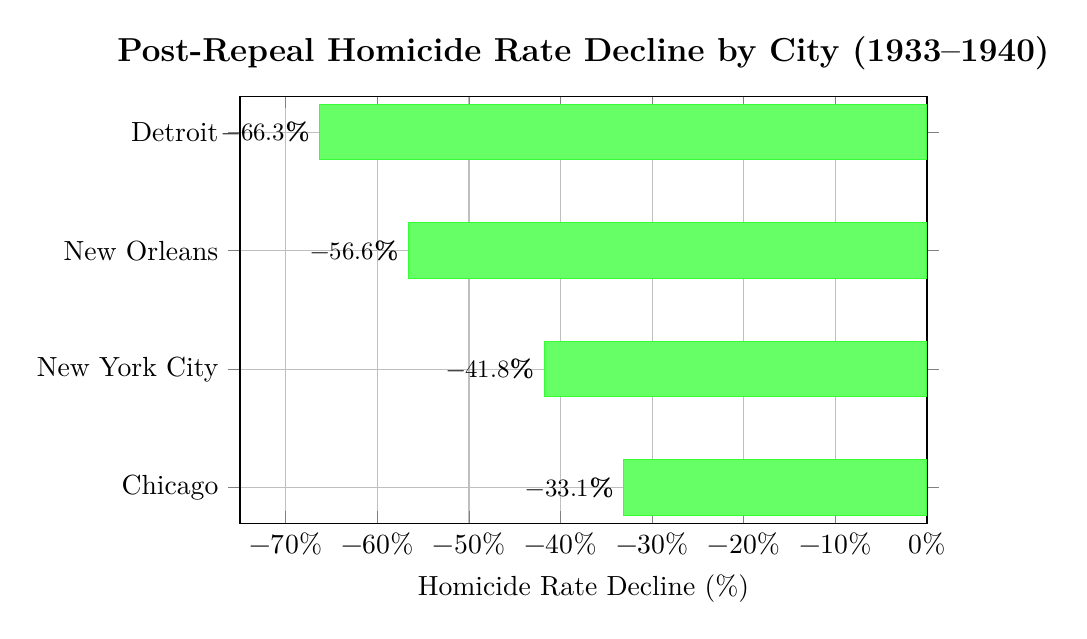
\begin{tikzpicture}
\begin{axis}[
    xbar,
    bar width=20pt,
    width=0.85\textwidth,
    height=7cm,
    xlabel={Homicide Rate Decline (\%)},
    symbolic y coords={Chicago,New York City,New Orleans,Detroit},
    ytick=data,
    y tick label style={font=\normalsize},
    xmin=-75, xmax=0,
    nodes near coords={\pgfmathprintnumber\pgfplotspointmeta\%},
    every node near coord/.append style={font=\small\bfseries, anchor=east},
    grid=major,
    title={\textbf{Post-Repeal Homicide Rate Decline by City (1933--1940)}},
    title style={font=\large},
    xticklabel={\pgfmathprintnumber\tick\%},
]
\addplot[fill=green!60, draw=green!80] coordinates {
(-33.1,Chicago)
(-41.8,New York City)
(-56.6,New Orleans)
(-66.3,Detroit)
};
\end{axis}
\end{tikzpicture}
\caption{The dramatic collapse in urban homicide rates following the repeal of Prohibition in 1933. Detroit, one of the primary border smuggling corridors from Canada, experienced the steepest decline (66.3\%). The sharp, synchronized drop across all major cities proves the violence was a direct structural output of the illicit market, not an endemic cultural condition. Sources: BJS Homicide Trends; CDC Vital Statistics.}
\label{fig:post-repeal-decline}
\end{figure}

\subsubsection{\texorpdfstring{\textbf{The Organizational Pivot of the
Underworld}}{The Organizational Pivot of the Underworld}}\label{the-organizational-pivot-of-the-underworld}

While the violence receded, the organizational infrastructure created by
Prohibition did not vanish; it adapted. The massive influx of capital
amassed during the 1920s provided mob bosses like Meyer Lansky, Frank
Costello, and the leaders of the Chicago Outfit with the resources to
transition into other highly lucrative, illicit fields.\\
The cartels seamlessly pivoted their sophisticated logistical networks
toward illegal gambling, extortion, labor union racketeering, and, most
consequentially, the burgeoning international narcotics trade. Former
rum-running fleets were repurposed for smuggling heroin and cocaine. The
vast wealth accumulated from bootlegging was also heavily invested in
the nascent, legal casino industry in Las Vegas by figures such as
Benjamin ``Bugsy'' Siegel and Moe Dalitz in the 1940s. Ultimately, while
Prohibition failed to dry up America, it succeeded in corporatizing the
American Mafia, providing them with the organizational blueprint and
financial war chest that would sustain their illicit operations for the
next half-century.\\
Simultaneously, the federal law enforcement apparatus that had been
rapidly expanded to fight the bootleggers and ``Public
Enemies''---specifically the FBI under J. Edgar Hoover and the Treasury
Department's Intelligence Units under Elmer Irey---retained their
enhanced budgets, personnel, and statutory authority. The bureaucratic
infrastructure built to wage the War on Crime in the 1930s became a
permanent fixture of the state, fundamentally shifting the balance of
police power from local municipalities to the federal government.

\begin{figure}[htbp]
\centering
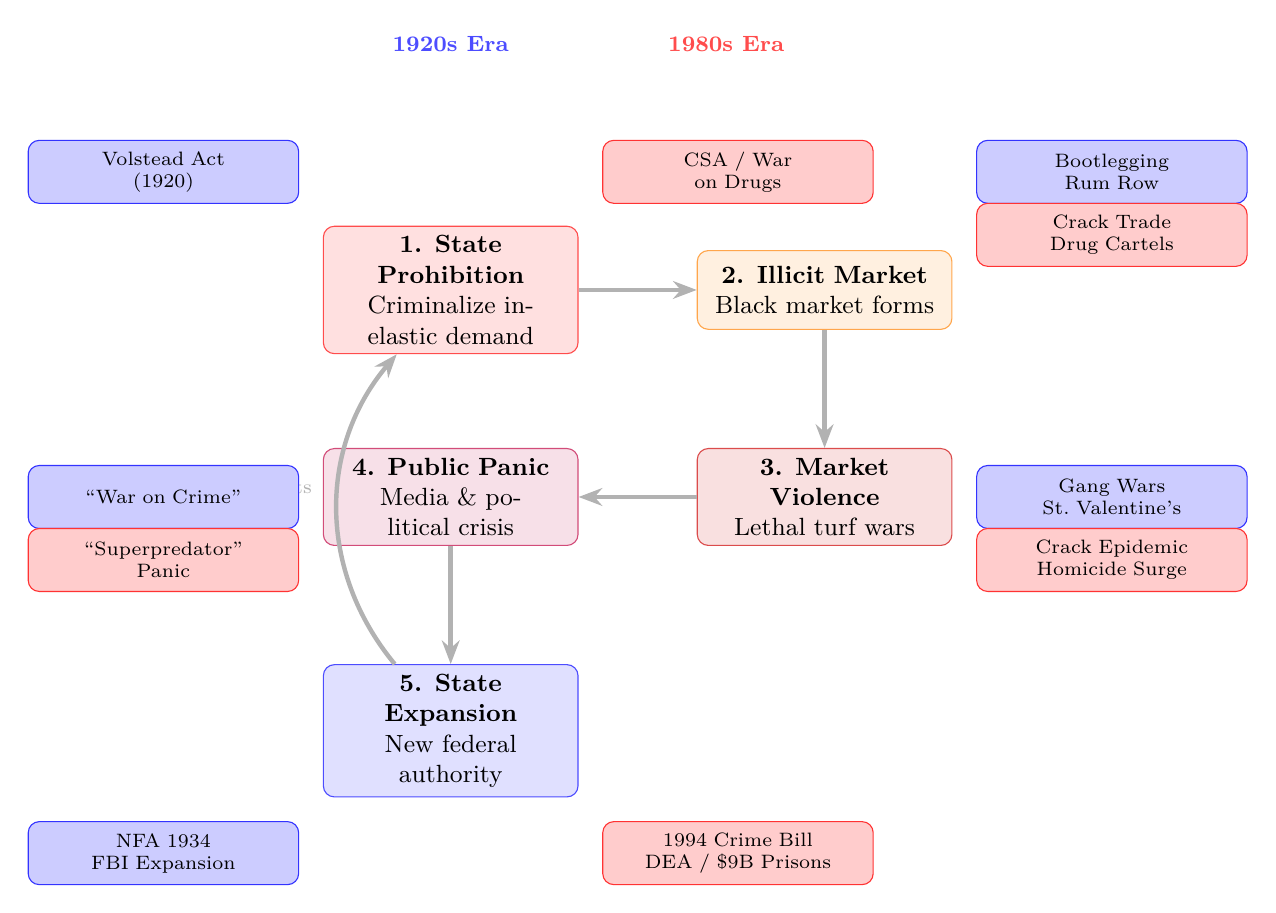
\begin{tikzpicture}[
    node distance=1cm and 0.6cm,
    every node/.style={font=\small},
    phase/.style={rectangle, draw=#1!70, fill=#1!12, text width=3cm, align=center, rounded corners, minimum height=1cm},
    cycle/.style={-{Stealth[length=3mm]}, ultra thick, gray!60},
    era/.style={rectangle, draw=#1!80, fill=#1!20, text width=3.2cm, align=center, rounded corners, minimum height=0.8cm, font=\scriptsize},
]

% Central cycle
\node[phase=red] (prohibit) {\textbf{1. State Prohibition}\\Criminalize inelastic demand};
\node[phase=orange, right=1.5cm of prohibit] (market) {\textbf{2. Illicit Market}\\Black market forms};
\node[phase=red!80!black, below=1.5cm of market] (violence) {\textbf{3. Market Violence}\\Lethal turf wars};
\node[phase=purple, left=1.5cm of violence] (panic) {\textbf{4. Public Panic}\\Media \& political crisis};
\node[phase=blue, below=1.5cm of panic] (expand) {\textbf{5. State Expansion}\\New federal authority};

% Cycle arrows
\draw[cycle] (prohibit) -- (market);
\draw[cycle] (market) -- (violence);
\draw[cycle] (violence) -- (panic);
\draw[cycle] (panic) -- (expand);
\draw[cycle, bend left=40] (expand) to node[midway, left, font=\scriptsize, text width=2cm, align=center] {Cycle repeats\\with new substance} (prohibit);

% 1920s track
\node[era=blue, left=0.3cm of prohibit, yshift=1.5cm] (e1a) {Volstead Act\\(1920)};
\node[era=blue, right=0.3cm of market, yshift=1.5cm] (e1b) {Bootlegging\\Rum Row};
\node[era=blue, right=0.3cm of violence] (e1c) {Gang Wars\\St.\ Valentine's};
\node[era=blue, left=0.3cm of panic] (e1d) {``War on Crime''};
\node[era=blue, below left=0.3cm and 0.3cm of expand] (e1e) {NFA 1934\\FBI Expansion};

% 1980s track
\node[era=red, right=0.3cm of prohibit, yshift=1.5cm] (e2a) {CSA / War\\on Drugs};
\node[era=red, right=0.3cm of market, yshift=0.7cm] (e2b) {Crack Trade\\Drug Cartels};
\node[era=red, right=0.3cm of violence, yshift=-0.8cm] (e2c) {Crack Epidemic\\Homicide Surge};
\node[era=red, left=0.3cm of panic, yshift=-0.8cm] (e2d) {``Superpredator''\\Panic};
\node[era=red, below right=0.3cm and 0.3cm of expand] (e2e) {1994 Crime Bill\\DEA / \$9B Prisons};

% Era labels
\node[font=\bfseries\footnotesize, blue!70] at ([yshift=2.3cm]prohibit.north) {1920s Era};
\node[font=\bfseries\footnotesize, red!70] at ([yshift=2.3cm, xshift=3.5cm]prohibit.north) {1980s Era};

\end{tikzpicture}
\caption{The recurring state algorithm identified across both prohibition eras: the state criminalizes inelastic demand, generating a violent black market, then leverages that violence to permanently expand federal police authority. The 1920s Alcohol Prohibition $\rightarrow$ NFA/FBI cycle was replicated precisely by the War on Drugs $\rightarrow$ 1994 Crime Bill/DEA cycle sixty years later. The cycle is self-reinforcing: expanded authority enables further prohibition, which generates further violence.}
\label{fig:prohibition-algorithm}
\end{figure}

\subsection{\texorpdfstring{\textbf{Conclusion}}{Conclusion}}\label{conclusion}

The violent saga of the Prohibition era stands as a premier historical
case study in the unintended, devastating externalities of absolute
legislative prohibition. By attempting to legislate morality and
engineer social purity through the Volstead Act, the United States
government inadvertently engineered a highly profitable, violently
competitive black market. This environment transformed decentralized,
local street gangs into formidable, heavily armed transnational
syndicates capable of rivaling the state in both wealth and localized
power.\\
The empirical data demonstrates that the historic surge in homicides
during the 1920s was not a failure of public morality or a symptom of
mass intoxication, but a predictable, structural output of an illicit
economy where lethal violence served as the sole available mechanism for
market regulation. When this violence reached an intolerable
zenith---typified by the public atrocity of the St.~Valentine's Day
Massacre---the state responded not by examining the root economic causes
of the violence, but by leveraging the crisis to aggressively expand its
regulatory reach. The passage of the National Firearms Act of 1934
established a foundational constitutional workaround, utilizing punitive
taxation to enact the nation's first sweeping federal gun control,
targeting the exact weapons the state's policies had made necessary for
criminal survival.\\
While the repeal of Prohibition in 1933 successfully collapsed the
homicide rate by removing the economic incentive for bootlegging
violence, the architectural legacy of the era remains permanently etched
into the nation's fabric. The ``noble experiment'' forged both the
sophisticated operational structure of the modern American Mafia and the
expansive, federalized law enforcement and gun control apparatus built
to combat it. Recognizing these interwoven frameworks through rigorous
historical analysis remains essential for understanding how state
interventions shape, accelerate, and occasionally institutionalize the
very violence they are theoretically designed to suppress.

\FloatBarrier
\nocite{*}
\printbibliography[title={Works cited},sorting=none]
\label{works-cited}

\end{document}
